% Sesi 2: integrasi Beamer dan overlay.
\documentclass[aspectratio=169]{beamer}
\usepackage{tikz}
\usetikzlibrary{positioning,arrows.meta}
\tikzset{tahap/.style={draw,rounded corners,fill=blue!10,minimum width=2.5cm,align=center},
 penting/.style={draw,rounded corners,fill=orange!20,minimum width=2.5cm,align=center}}
\begin{document}
\begin{frame}{Alur penelitian: tampil bertahap}
\centering
\begin{tikzpicture}[node distance=1.4cm]
\node[tahap] (a) {Pertanyaan};
\node[tahap,right=of a] (b) {Metode};
\node[penting,right=of b] (c) {Temuan};
\only<2->{\draw[-{Stealth},thick] (a) -- (b);}
\only<3->{\draw[-{Stealth},thick] (b) -- (c);}
\begin{scope}[yshift=-1.2cm]
\node[align=center] at (b) {Anotasi: pilih metode sesuai pertanyaan};
\end{scope}
\end{tikzpicture}
\par\medskip\small Gambar: contoh hubungan pertanyaan, metode, dan temuan.
\end{frame}\end{document}
